\section{Path Planning}\label{sec:path_planning}

The third major component of the path execution subsystem is a path planner. This component sits above the trajectory generation component and takes goals from other robot subsystems and outputs paths that the precision navigation system should follow. The path planner fills a similar role to that of the navfn described in \autoref{subsec:navfn}. The output is an ordered sequence of path segments (see \autoref{subsec:path_segment} for the detailed description of a path segment) that must be blended smoothly such that there are no discontinuities in position or orientation between the end of one segment and the beginning of the next segment.

\begin{figure}
\centering
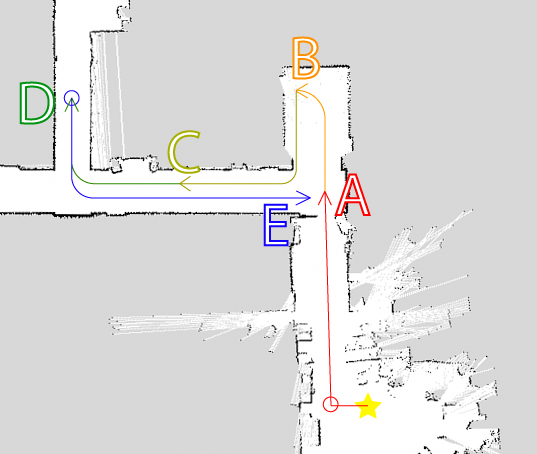
\includegraphics[width=0.75\textwidth]{images/2nd_floor_one_door_cropped_annotated}
\caption[Annotated Goals with Pre-planned Paths Example]{Annotated Goals with Pre-planned Paths Example. This is the second floor of the CWRU Glennan building. Each separate path segment is in a different color. Goals are annotated with a letter in the same color as the path leading to that goal. Circles are spin-in-place segment locations. Arrows indicate the direction of the paths. The star is the intended initial robot pose, which is in the Glennan 210 Robotics Lab \label{fig:annotated_path_example}}
\end{figure}

While a complete path planning system able to generate blended paths to arbitrary goals in arbitrary environments was beyond the scope of this thesis, a minimal path planner for using the precision navigation system on \emph{a priori} paths to pre-defined goals with limited capability for replanning around dynamic obstacles was developed. This minimal path planner was used to validate the performance of the other precision navigation components in an autonomous system, where the only human action required is the selection of a destination location. See \autoref{fig:annotated_path_example} for an example of a set of pre-planned paths with corresponding annotated goals (simply A, B, C, etc. in this example but they could easily be ``elevator'' or ``bathroom''). Possible extensions to this minimal path planner are discussed in \autoref{sec:future_work}.

The path planner developed in this thesis has a number of assumptions about its environment. It should be noted that none of these assumptions are necessarily required for precision navigation with a sufficiently advanced path planning component and are specific to the limited path planner developed in this thesis. The first assumption is, in addition to an \emph{a priori} obstacle map of static obstacles, this map will be annotated with goal locations and that there is an ordered sequence of path segments describing how to get from one goal to another. These goal locations and pre-planned paths are the only paths that the planner can send to the rest of the precision navigation system. For this thesis, the goals were selected to be ``interesting'' destination locations for a smart wheelchair, such as ``elevator'' or ``bathroom''. The paths between these goal locations were generated by driving the robot along the desired path while recording control points along the path. These control points were then split into different path segments and the geometric parameters were fit to each segment's control points using Matlab. For example, for a constant curvature arc segment, four control points were required in order to solve for the circular arc that blends a pair of lines defined by those four control points. Parameters such as maximum speed and acceleration limits were inserted by hand based on desired behavior and HARLIE's safety limits.

The next set of assumptions is related to the initial conditions of the robot when a given pre-planned path is selected. Firstly, the path planner assumes that, when a given path is commanded, the robot is at the origin of the first path segment, as there is no automatic segment generation to connect the current robot pose to the origin of the commanded path. If the robot is not near the origin of the path when the path is commanded, whether the robot will be able to complete the path depends on the steering algorithm's attraction region, as the desired states output by the trajectory planner will always lie on a path segment. If the robot's pose is within the steering algorithm's attraction region, the robot will eventually converge onto the commanded path and precisely follow it; if the robot's pose is outside the attraction region, it is unlikely that the robot will converge on the commanded path. Even if the robot is within the steering algorithm's attraction region, there is a second condition that must be satisfied if the robot is to converge onto the path: the space between the robot's current pose and the origin of the path must be free of obstacles. Because the path planner does not plan between the robot's current pose to the origin of the path, it cannot replan around obstacles between the robot and the origin of the path. In a normal use case, this condition is not difficult to satisfy if the robot navigated to the origin of the path using a different path; for example, if the robot first went to the ``elevator'' and then took the path between the ``elevator'' and ``bathroom'' in order to get to the bathroom, then it should have ended up very close to the origin of the ``elevator'' to ``bathroom'' pre-planned path and it is unlikely that there would be any obstacles within a short distance (ten centimeters or so) of a goal point. Another use case, where a human has to position the robot near to the origin of a desired path before sending the planner a goal has a similar assumption -- it is unlikely that a human, manually positioning the robot, would position it such that there is an obstacle between the robot and the origin of the path.

Even with these limitations, the path planner developed for this thesis was sufficient for precisely navigating in static indoor environments. In order to validate that dynamic replanning around obstacles was possible within the framework of the precision navigation system, the path planner was extended with the ability to ``splice'' in a sequence of path segments to go around the dynamic obstacle encountered. The splicing, which takes place whenever an imminent collision is detected by the trajectory generation, is made up of the following steps:

\begin{enumerate}
\item Wait for $n$ seconds, aborting splicing if there will no longer be a collision (e.g. if a person was simply walking across the robot's path)
\item Confirm the desired state (with forward simulation along the path segment) will still cause a collision
\item Shorten the current path segment to end at the current desired state
\item Add the following path segments to the path between the shortened current path segment and the next segment of the original path
	\begin{enumerate}
	\item Spin-in-place $\frac{\pi}{2}$ radians to be orthogonal to the original path segment
	\item Semicircle with a one meter radius
	\item Spin-in-place $\frac{\pi}{2}$ radians to the orientation of the current path segment
	\item Add a straight line segment from the last spin-in-place to the next segment
	\end{enumerate}
\item Send path with spliced segments and the remainder of the original path to the trajectory generator
\end{enumerate}

While these splicing steps are somewhat limited in that they assume that the obstacle will either move out of the way (the reason for waiting for $n$ seconds, fifteen in this thesis, before splicing) or that a semicircle with a one meter radius will be sufficient to go around the obstacle. Though the splicing behavior is a rather primitive method of replanning to avoid dynamic obstacles, it was sufficient to function as a proof-of-concept that the precision navigation system can avoid dynamic obstacles.

\begin{comment}

\begin{enumerate}
\item Annotated or not map?
\item Initial conditions?
\item Friendly assumptions about initial clear path?
\item How to account for dynamic obstacles that invalidate our original plan (those bastards...).
\end{enumerate}

\end{comment}
